\documentclass[presentation,aspectratio=169]{beamer}
\usepackage[utf8]{inputenc}
\usepackage[T1]{fontenc}
\usepackage{graphicx}
\graphicspath{{./graphics/}}
\usepackage[ngerman]{babel}
\usepackage{longtable,capt-of,fvextra,csquotes}
\usepackage{wrapfig,rotating}
\usepackage[normalem]{ulem}
\usepackage{amsmath,amssymb}
\usepackage{hyperref}
\usepackage{listings,minted}
\usepackage[duration=20]{pdfpc}
\usetheme{metropolis}
\author{Julius Freudenberger}
\date{Hackathon Sommersemester 2022}
\title{WYSIWYAF with \LaTeX}
\mode<presentation>{\usetheme{metropolis}}
\mode<beamer|handout>{\metroset{sectionpage=progressbar}}
\mode<beamer|handout>{\metroset{subsectionpage=progressbar}}
\mode<beamer|handout>{\metroset{block=fill}}
\institute[Hochschule Esslingen]{Hochschule Esslingen}
\hypersetup{
  pdfauthor={Julius Freudenberger},
  pdftitle={WYSIWYAF with LaTeX},
  pdfkeywords={},
  pdfsubject={},
  pdflang={German},
  colorlinks,
  linkcolor=black,
  citecolor=black,
  filecolor=black,
  urlcolor=blue
}
\usepackage{biblatex}

\begin{document}

\maketitle

\begin{frame}[fragile]{Bevor wir beginnen: Was brauche ich?}
  \begin{itemize}
    \item \LaTeX-Distribution: \TeX{}Live
      \begin{itemize}
        \item Windows: \href{https://tug.org/texlive/windows.html}{https://tug.org/texlive/windows.html} %TODO MikTeX?
        \item Mac: \href{https://tug.org/mactex/}{https://tug.org/mactex/}
        \item Linux: Installation über den Paketmanager
          \begin{itemize}
            \item deb: \verb|texlive-base| (deb), \verb|texlive texlive-latex| (rpm)
            \item Arch Linux: \verb|texlive-core|
            \item NixOS: \verb|nixpkgs.texlive.combined.scheme-basic|
          \end{itemize}
        \item Docker: \verb|texlive/texlive|
      \end{itemize}
    \item Texteditor
      \begin{itemize}
        \item VSCode mit \LaTeX-Workshop, vim mit vimtex
        \item \href{https://www.xm1math.net/texmaker/index.html}{\TeX{}Maker}
      \end{itemize}
    \item Alternativ: Online-Editoren
      \begin{itemize}
        \item Overleaf (\href{https://www.overleaf.com}{https://www.overleaf.com}, Registrierung erforderlich)
        \item \TeX{}Viewer (\href{https://texviewer.herokuapp.com}{https://texviewer.herokuapp.com}, direkt nutzbar)
      \end{itemize}
  \end{itemize}
\end{frame}

\begin{frame}{Was ist \LaTeX?}
  \pdfpcnote{ - Entwicklung seit Anfang der 1980er
  - What you see is what you get --> What you see is what you asked for}
  \begin{itemize}
    \item Textsatzsystem
    \item setzt vorgegebenen Text und weitere Anweisungen automatisch
    \item versucht automatisch bestmögliches Layout
    \item kein WYSIWYG, sondern WYSIWYAF
    \item Quellcode wird \glqq{}kompiliert\grqq{}
    \item Dokument wird als PDF, PS, DVI oder sogar HTML ausgegeben
  \end{itemize}
\end{frame}

\begin{frame}{Warum \LaTeX?}
  \pdfpcnote{ Vergleich zu Word
    - schöner Blocksatz, bestmögliche Zeilenumbrüche und Worttrennungen
    - Inhaltsverzeichnis und Verzeichnisse für Abbildungen, Stichworte, Abkürzungen und Literatur
    - Abbildungen und weitere Referenzelemente werden automatisch an der bestmöglichen Stelle eingefügt
  - Deutlich mehr Automatisierungen als bei Word, "Layoutarbeit" am Ende einer Arbeit deutlich geringer}
  \begin{itemize}
    \item Automatischer Textsatz
    \item Automatische Referenzen
    \item Automatisches Layout
  \end{itemize}
\end{frame}

\begin{frame}{Wie sieht \LaTeX-Code aus?}
  \pdfpcnote{
    - Befehle werden mit \ angegeben
    - Parameter mit {}
    - Einrückung hilft bei Lesbarkeit, ist nicht notwendig
    - Beginn und Ende
    - normaler Text
  }
  \inputminted{latex}{codebeispiele/beispiel.tex}
\end{frame}

\begin{frame}{Grundlegender Aufbau}
  \pdfpcnote{
    - Dokumentenklasse (book, article, beamer)
    - Präambel
    - Metadaten (Titel, Autor, Datum)
    - Zusätzliche Pakete
    - Einstellungen
    - Eigentliches Dokument
  }
  \inputminted{latex}{codebeispiele/aufbau.tex}
\end{frame}

\begin{frame}{Vorlage herunterladen}
  \begin{itemize}
    \item \href{https://www2.hs-esslingen.de/~jufrit00/latex/}{https://www2.hs-esslingen.de/\textasciitilde{}jufrit00/latex/}
    \item \href{https://gitlab.hs-esslingen.de/jufrit00/latex-workshop}{https://gitlab.hs-esslingen.de/jufrit00/latex-workshop}
    \item \href{https://github.com/JuliusFreudenberger/latex-workshop}{https://github.com/JuliusFreudenberger/latex-workshop}
  \end{itemize}
\end{frame}

\begin{frame}[fragile]{Projekt kompilieren}
  \begin{itemize}
    \item Im Projektverzeichnis \verb|pdflatex file.tex|
    \item automatisierter mit \verb|latexmk -pdf file.tex|
    \item In \TeX{}Maker \glqq{}Schnelles Übersetzen\grqq{}
    \item mittels Docker und Docker Compose (Anleitung im Git Repo)
    \item Outputfile \verb|file.pdf| als PDF-Datei im gleichen Verzeichnis
  \end{itemize}
\end{frame}

\begin{frame}[fragile]{Erste eigene Änderungen}
  \pdfpcnote{
    - Stärke von LaTeX: Änderungen wirken sich konsistent auf das gesamte Dokument aus.
    - Keine manuelle Anpassung an mehreren Stellen nötig.
    - Niedrigste Stufe: subsubsection
    - Bei Text am Besten ein Satz in eine Zeile.
  }
  \begin{itemize}
    \item Eigener Text, Absätze
    \item Textformatierung: \textbf{fett} und \textit{kursiv} mit \verb|\textbf{fett}|, \verb|\textit{kursiv}|
    \item Eigene Abschnitte mit \verb|\section{} und \subsection{}|
    \item Metadaten ändern
      \begin{itemize}
        \item Titel des Dokuments ändern mit \verb|\title{}|
        \item Eigener Name als Autor mit \verb|\author{}|
      \end{itemize}
  \end{itemize}
\end{frame}

\begin{frame}[fragile]{Umgebungen}
  \begin{itemize}
    \item kennzeichnen besondere Bereiche im Dokument
    \item beginnen mit \verb|\begin{}| und enden mit \verb|\end{}|
    \item können verschachtelt werden, aber nicht geschnitten
    \item Aufzählungen \verb|enumerate| (nummeriert) und \verb|itemize| (unnummeriert)
  \end{itemize}
  \begin{center}
    \centering
    \begin{minted}{latex}
\begin{itemize}
  \item Erster Punkt
  \item Zweiter Punkt
\end{itemize}
    \end{minted}
  \end{center}
\end{frame}

\begin{frame}[fragile]{Wichtige besondere Zeichen}
  \begin{tabular}{c|c|c}
    Schrägstrich                                  & \textbackslash   & \verb|\textbackslash| \\
    \hline
    Tilde                                         & \textasciitilde  & \verb|\textasciitilde| \\
    \hline
    geschütztes Leerzeichen (ohne Zeilenumbruch)  & ~                & \verb|~| \\
    \hline
    schmales geschütztes Leerzeichen              & z.\,B.           & \verb|z.\,B.| \\
    \hline
    Gedankenstrich (Halbgeviertstrich)            & --               & \verb|--| \\
    \hline
    Geviertstrich                                 & ---              & \verb|---|
  \end{tabular}
\end{frame}

\begin{frame}[fragile]{Verweise}
  \begin{itemize}
    \item Label setzen: \verb|\label{<name>}|
    \item Abschnitt referenzieren: \verb|\ref{<name>}|
    \item Seite referenzieren: \verb|\pageref{<name>}|
    \item Referenz nutzt immer aktuellste Abschnittnummer und Seitenzahl
    \item zur Aktualisierung doppelte Durchläufe notwendig
  \end{itemize}
\end{frame}

\begin{frame}{Mathematik}
  \begin{itemize}
    \item \TeX{} ist für seine gute Formeleingabe bekannt
    \item verschiedene Modi, in denen Formeln gesetzt werden können
      \begin{itemize}
        \item inline
        \item Block
        \item Gleichung
      \end{itemize}
  \end{itemize}
\end{frame}

\begin{frame}[fragile]{Mathematik --- inline}
  \begin{itemize}
    \item setzt die Gleichung in einen Fließtext ein
    \item keine Referenzierung
    \item Beginn und Ende mit \verb|$|
  \end{itemize}
  
  \begin{minipage}{.4\textwidth}
    Hier ist nun ein Fließtext,
in den ich eine Gleichung
$f(x)=x^2$ setzen möchte.

  \end{minipage}
  \hfill
  \begin{minipage}{.5\textwidth}
    \inputminted{latex}{codebeispiele/math-inline.tex}
  \end{minipage}
\end{frame}

\begin{frame}[fragile]{Mathematik --- block}
  \begin{itemize}
    \item setzt die Gleichung als Block mit Absätzen
    \item keine Referenzierung
    \item Beginn mit \verb|\[|, Ende mit \verb|\]|
  \end{itemize}
  
  \begin{minipage}{.4\textwidth}
    In diesem Absatz geht es 
um ein wichtiges Thema.
Nun folgt eine Gleichung:
\[f(x)=x^2\]
In dieser Gleichung ist
eine wichtige Information!

  \end{minipage}
  \hfill
  \begin{minipage}{.5\textwidth}
    \inputminted{latex}{codebeispiele/math-block.tex}
  \end{minipage}
\end{frame}

\begin{frame}[fragile]{Mathematik --- Gleichung}
  \begin{itemize}
    \item setzt die Gleichung als Block mit Absätzen
    \item Referenzierung über Nummerierung
    \item Beginn mit \verb|\begin{equation}| Ende mit \verb|\end{equation}|
  \end{itemize}
  
  \begin{minipage}{.4\textwidth}
    Hier ist eine Gleichung:
\begin{equation}\label{gleichung}
  f(x)=x^2
\end{equation}
In Gleichung \eqref{gleichung}
geht es um \dots

  \end{minipage}
  \hfill
  \begin{minipage}{.5\textwidth}
    \inputminted{latex}{codebeispiele/math-equation.tex}
  \end{minipage}
\end{frame}

\begin{frame}[fragile]{Mathematik --- Zeichen}
  \begin{minipage}{.4\textwidth}
    \begin{align}
  f(x)=x^2\\
  f_{xy}(x)=x^{2-y}\\
  \pi \approx 3,14\\
  2 \cdot{} 4 \leq 8\\
  1 < 2 > 1, 2 \neq 3\\
  (f^{-1}_{x})\\
  \left(f^{-1}_{x}\right)\\
  \sqrt{16}=4, \sqrt[4]{64}=2
\end{align}

  \end{minipage}
  \hfill
  \begin{minipage}{.5\textwidth}
    \inputminted{latex}{codebeispiele/math-symbols.tex}
  \end{minipage}
\end{frame}

\begin{frame}[fragile]{Abbildungen und Graphiken}
  \begin{itemize}
    \item Paket \verb|graphicx|
    \item Unterstützung von jpg, png und pdf, Dateiendung kann weggelassen werden
    \item Höhe und Breite als optionale Parameter
      \begin{itemize}
        \item \verb|\textwidth| oder \verb|textheight|
      \end{itemize}
    \item
      \begin{minted}{latex}
\includegraphics[width=.5\textwidth]{<filename>}
      \end{minted}
  \end{itemize}
  \begin{center}
    
\includegraphics[height=.5\textheight]{katze}
  \end{center}
\end{frame}

\begin{frame}{Graphiken als Gleitobjekt}
  \begin{itemize}
    \item Automatische Positionierung im Text
    \item Referenzierung mit Nummerierung über Label
  \end{itemize}
  \begin{minipage}[c]{.4\textwidth}
    \begin{figure}
  
\includegraphics[width=
  .7\textwidth]{katze}
  \caption{Eine Katze}
  \label{fig:katze}
\end{figure}
Abbildung \ref{fig:katze}
zeigt eine Katze.

  \end{minipage}
  \hfill
  \begin{minipage}[c]{.5\textwidth}
    \inputminted{latex}{codebeispiele/graphics-figure.tex}
  \end{minipage}
\end{frame}

\begin{frame}[fragile]{Codelistings}
  \begin{itemize}
    \item Abdrucken von Codezeilen
    \item Syntaxhighlighting und Zeilennummern
    \item mögliche Pakete
      \begin{itemize}
        \item \verb|verbatim|
        \item \verb|listings|
        \item \verb|minted|
      \end{itemize}
  \end{itemize}
\end{frame}

\begin{frame}[fragile]{Die verbatim-Umgebung}
  \begin{itemize}
    \item kein Syntaxhighlighting und Zeilennummern
    \item Monospacefont
    \item Befehle werden nicht ausgeführt
  \end{itemize}
  \begin{minipage}{.4\textwidth}
    \verb|Text in Monospacefont|.

\begin{verbatim}
Absatz in Monospacefont.
Hier könnte Code dargestellt
werden.
\end{verbatim}

  \end{minipage}
  \hfill
  \begin{minipage}{.5\textwidth}
    \inputminted{latex}{codebeispiele/listings-verbatim.tex}
  \end{minipage}
\end{frame}

\begin{frame}[fragile]{Die lstlistings-Umgebung}
  \begin{itemize}
    \item Syntaxhighlighting bestimmter Sprachen und Zeilennummern
    \item Customization mit Schriftgröße und Farben
  \end{itemize}
  \begin{minipage}{.4\textwidth}
    \begin{lstlisting}[language=java]
public void main() {
  System.out.println("Hi");
}
\end{lstlisting}

  \end{minipage}
  \hfill
  \begin{minipage}{.5\textwidth}
    \inputminted{latex}{codebeispiele/listings-lstlistings.tex}
  \end{minipage}
\end{frame}

\begin{frame}[fragile]{Die minted-Umgebung}
  \begin{itemize}
    \item Syntaxhighlighting vieler Sprachen
    \item Farben direkt voreingestellt
    \item benötigt \verb|pygmentize| und \verb|shell-escape|-Option beim Kompilieren
  \end{itemize}
  \begin{minipage}{.4\textwidth}
    \begin{minted}{java}
public void main() {
  System.out.println("Hi");
}
\end{minted}

  \end{minipage}
  \hfill
  \begin{minipage}{.5\textwidth}
    \inputminted{latex}{codebeispiele/listings-minted.tex}
  \end{minipage}
\end{frame}

\begin{frame}[fragile]{Code aus Datei einbinden}
  \begin{itemize}
    \item besonders geeignet für längere Codeauszüge
  \end{itemize}
  \begin{minipage}{.4\textwidth}
    \lstinputlisting[language=java]
{codebeispiele/example.java}

\inputminted{java}
{codebeispiele/example.java}

  \end{minipage}
  \hfill
  \begin{minipage}{.5\textwidth}
    \inputminted{latex}{codebeispiele/listings-from-file.tex}
  \end{minipage}
\end{frame}

\begin{frame}[fragile]{Weitere Verzeichnisse}
  \begin{itemize}
    \item automatisch aktualisierendes Inhaltsverzeichnis sowie Verzeichnisse für Abbildungen, Codelistings (Abkürzungen, Stichwörter, Bibliographie, \dots)
  \end{itemize}
  \inputminted{latex}{codebeispiele/list-of-everything.tex}
\end{frame}

\begin{frame}{Nächste Projekte für \LaTeX{}?}
  \begin{itemize}
    \item Wissenschaftliches Dokumentieren
    \item Praxissemesterbericht
    \item Thesis
    \bigskip
    \item Bewerbungsunterlagen
  \end{itemize}
\end{frame}

\begin{frame}[fragile]{Bewerbungsunterlagen}
  \begin{itemize}
    \item Lebenslauf mit \verb|moderncv|
    \item Anschreiben mit \verb|dinbrief|
  \end{itemize}
  \begin{center}
    
\includegraphics[height=.7\textheight]{Lebenslauf}
    \hspace{1em}
    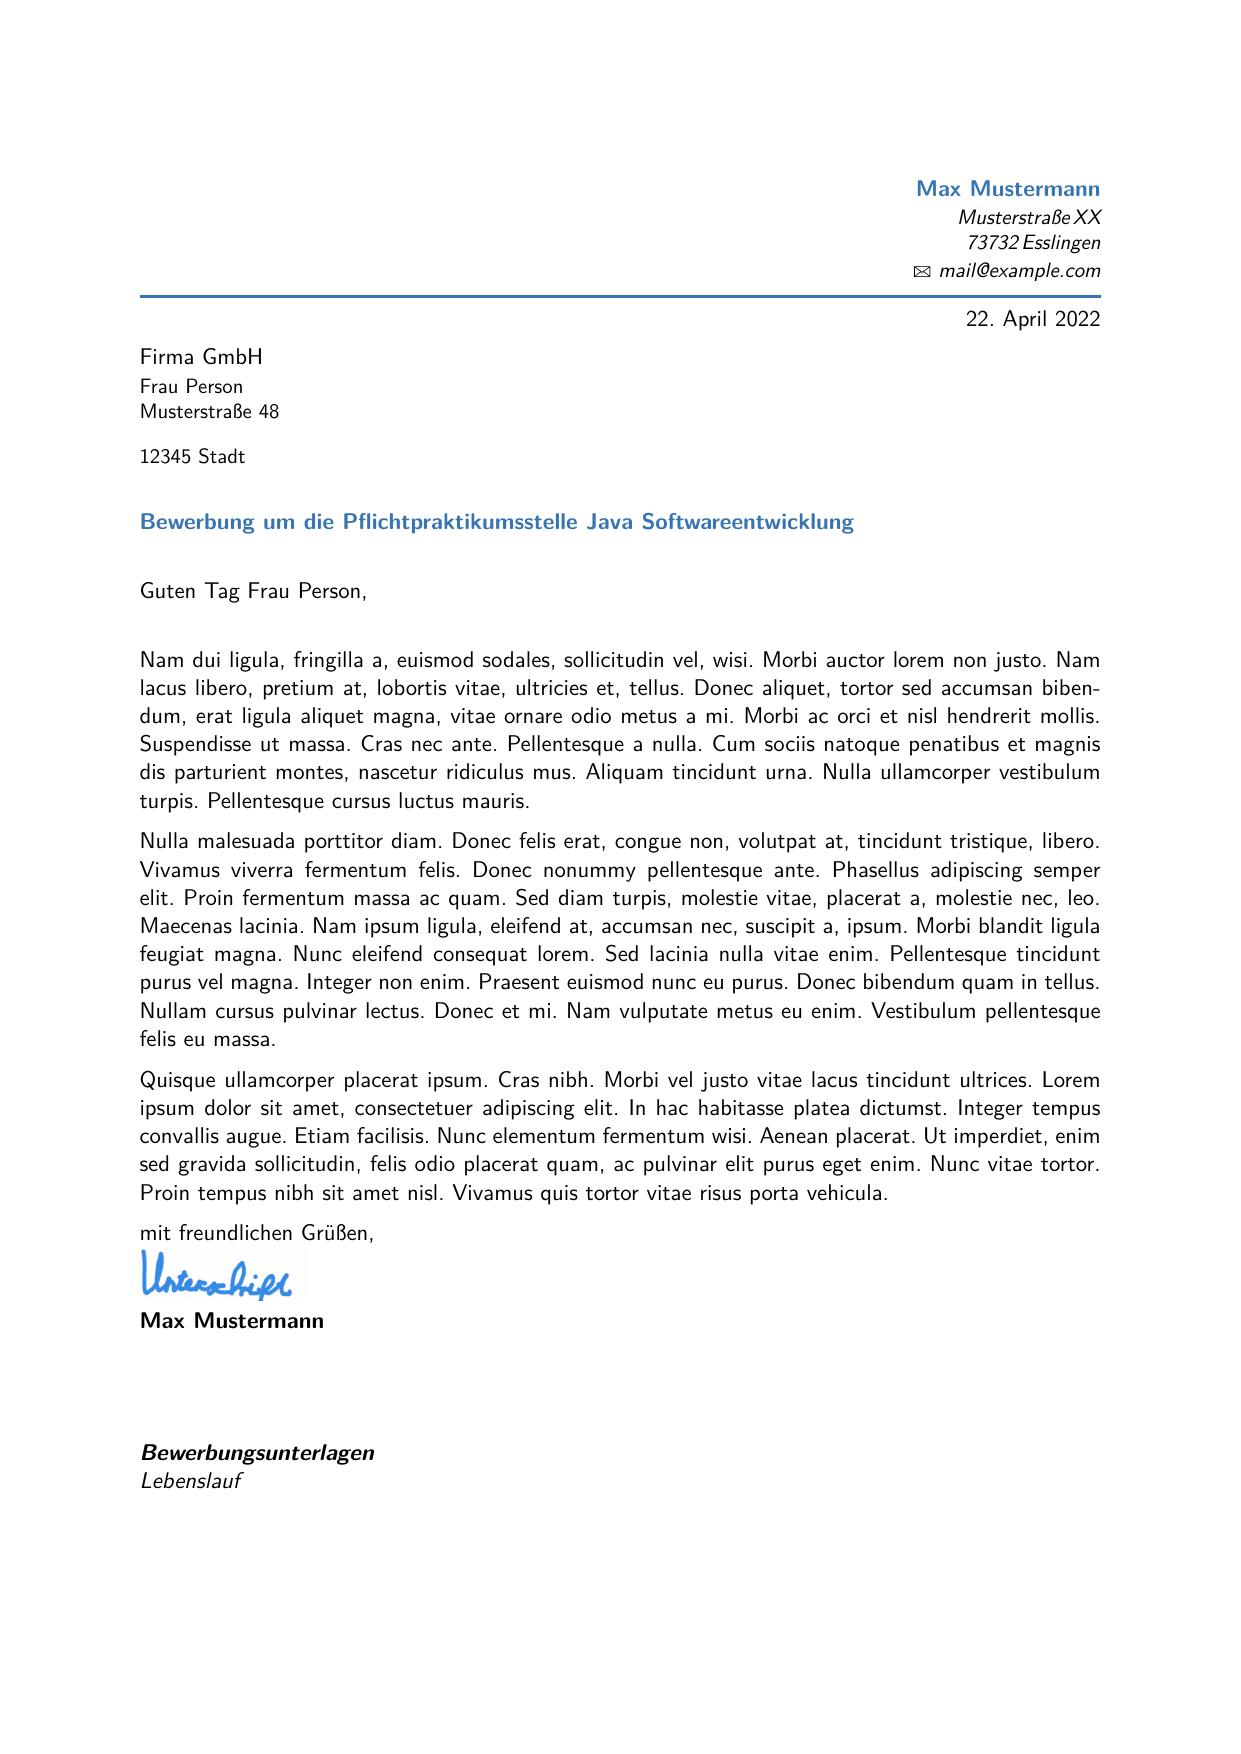
\includegraphics[height=.7\textheight]{Anschreiben}
  \end{center}
\end{frame}

\begin{frame}{Wohin bei Problemen?}
  \begin{itemize}
    \item Suchmaschine des Vertrauens
    \item \href{https://de.wikibooks.org/wiki/LaTeX-Kompendium}{\LaTeX-Kompendium}
    \item \href{https://www.overleaf.com/learn}{Overleaf documentation}
    \item \href{https://golatex.de/wiki/index.php/Hauptseite}{Go\LaTeX-Wiki}
    \item \href{https://tex.stackexchange.com}{\TeX-Stackexchange}
  \end{itemize}
\end{frame}

\maketitle

\end{document}
